\section{Entscheidungsbäume, Boosting und Bagging}
\textit{Annalena Gutheil, Matthias Volland}

Die Verwendung von baumartigen Strukturen zur Klassifikation von Daten bietet sich aus mehreren Gründen an. 
Einerseits handelt es sich bei Bäumen um eine Datenstruktur, die häufig in der Informatik verwendet wird und daher 
vom Verständnis intuitiver ist, als beispielsweise ein neuronales Netzwerk oder eine SVM. 
Andererseits ist das Erzeugen von Bäumen im Allgemeinen relativ effizient, was bei Machine-Learning-Algorithmen 
in der Traningsphase wichtig ist. Das Verwenden bzw. Durchlaufen eines Baumes hat lediglich eine logarithmische Komplexität, 
so dass auch die Klassifikation durch einem Baum sehr effizient ist, sofern dieser nicht entartet ist. 

\subsection*{Entscheidungsbäume}

Bäume zur Klassifikation von Daten werden auch als \glqq Entscheidungsbäume\grqq\ bezeichnet und bestehen aus Knoten, Kanten und Blättern. Knoten entsprechen dabei Merkmalen bzw. \glqq Features\grqq\ der zu klassifizierenden Daten und die Kanten an einem Knoten den verschiedenen Merkmalsausprägungen. 
Ein Knoten kann entweder einen weiteren Knoten als Kind haben (also ein weiteres Merkmal) oder aber ein Blatt, was einer Klasse entspricht.

Um beispielsweise verschiedene Gemüsesorten zu klassifizieren, könnten im einfachsten Fall Farbe und Form als Unterscheidungsmerkmale dienen. Wenn jedes Objekt der Testmenge die Merkmale (Form, Farbe) hat, würde eine Tomate mit (rund, rot) beschrieben, eine Gurke mit (länglich, grün) und eine Möhre mit (länglich, orange).

Ein Entscheidungsbaum zur Klassifikation könnte dann aus einem Wurzel-Knoten bestehen, der zunächst anhand der Form 
des zu klassifizierenden Objektes eine erste Entscheidung vornimmt. Da eine Tomate rund ist und Gurken und Möhren länglich, 
hätte der Wurzelknoten zur Unterscheidung der Form die beiden Kanten \glqq rund\grqq\ und \glqq länglich\grqq\ . Da in dem Beispiel nur Tomaten rund sind, hätte die Kante mit dem Attribut \glqq rund\grqq\ das Blatt bzw. die Klasse \glqq Tomate\grqq\ als Kind. Gurken und Möhren haben 
jedoch beide eine längliche Form, so dass diese nicht alleine aufgrund der Form unterschieden werden können. Daher müsste die 
Kante mit dem Merkmal \glqq länglich\grqq\ in einen weiteren Knoten münden, durch welchen die Testmenge in einem nächsten Schritt anhand der Farbe weiter unterteilt werden müsste. Dieser Entscheidungsknoten hätte die Kanten \glqq rot\grqq , \glqq grün\grqq\ und \glqq orange\grqq, die jeweils in einem Blattknoten mit den Klassen \glqq Tomate\grqq , \glqq Gurke\grqq\ und \glqq Möhre\grqq\ müden würden.

In dem Beispiel hätte als erstes Unterscheidungsmerkmal auch die Farbe dienen können, wodurch direkt in einem Schritt alle drei Gemüsesorten hätten klassifiziert werden können. Somit hat die Wahl der Reihenfolge der Merkmale einen wesentlichen Einfluss auf die Form des Entscheidungsbaumes sowie die Effizienz, mit der Testdaten klassifiziert werden können. Weiterhin können durch die ungünstige Wahl von Kriterien verschiedene Klassen mehrfach in dem Entscheidungsbaum vorkommen, was darauf schließen lässt, dass der Baum aufgrund der Redundanz mehr Knoten enthält, als für eine Klassifizierung notwendig wäre.

Es gibt verschiedene Kriterien, nach denen die Reihenfolge der Merkmale so gewählt werden kann, dass ein möglichst kompakter und damit effizienter Entscheidungsbaum entsteht. Ein Ansatz besteht darin zu berechnen, wie groß der Informationsgehalt der zu unterscheidenden Merkmale ist. Da sich durch das Merkmal \glqq Farbe\grqq\ aus dem vorigen Beispiel direkt alle möglichen Klassen unterscheiden lassen, hat dieses Merkmal z.B. einen höheren Informationsgehalt als das Merkmal \glqq Form\grqq\ und bietet sich daher als erstes Entscheidungskriterium an. Dieser Informationsgehalt wird auch als \glqq Entropie\grqq\ bezeichnet.
Ein anderes Maß zur Auswahl von geeigneten Entscheidungsmerkmalen ist die sogenannte \glqq Reinheit\grqq\ von Merkmalen. Die Reinheit eines Merkmales ergibt sich daraus, wie viele verschiedene Klassen die jeweiligen Merkmalsausprägungen beinhalten. Das Attribut \glqq Farbe\grqq\ aus dem vorigen Beispiel führt zu drei Blattknoten, bei denen durch jeden Knoten genau eine Klasse repräsentiert wird (nämlich jeweils die Klassen Tomate, Gurke und Möhre) während beim Merkmal \glqq Form\grqq\ sowohl Möhren als auch Gurken als mögliches Ergebnis in Frage kommen, falls das zu klassifizierende Objekt die Merkmalsausprägung \glqq länglich\grqq\ hat. 

%Entscheidungsbäume funktionieren nach dem \glqq teile und herrsche\grqq\ -Prinzip. 
%Beginnend beim Wurzelknoten wird bei jedem Knoten mithilfe einer Testfunktion berechnet, welche Abzweigung genommen werden muss. 
%Ist man am Blattknoten angekommen, ist dies die zur Eingabe gehörende Klasse~\cite{alpaydin:maschinelles_lernen, borgelt:data_mining}.

\subsection*{Random Forests}

Die Besonderheit von Ensemble Learning ist, dass mit Hilfe von vielen schwachen Klassifikatoren 
gute Klassifikationsergebnisse erzielt werden können. 
Die Entscheidungen, die die verschiedenen Klassifikatoren treffen, sind dabei verschieden, 
was jedoch auch die Stärke dieser Methode ist, denn sie ergänzen sich gegenseitig

\subsection{Datenaufbereitung}

Die zu klassifizierenden Gesten unterscheiden sich dahingehend, dass sie die Bandbreite 
des Frequenzspektrums um den Referenzton in unterschiedlicher Weise verschieben bzw. vergrößern. 
Um eine Geste zu erkennen, werden daher die Amplituden der aufgezeichneten Frequenzen 
um die Amplitude der Frequenz des Referenztons im Spektrum in beiden Richtungen analysiert. 
Relevant für die Erkennung der Gesten sind dabei im Allgemeinen nur diejenigen Frequenzanteile 
um den Referenzton, deren Amplitude den Grenzwert von 10\% der Amplitude des Referenztones nicht unterschreitet. 
In Ausnahmefällen können die Frequenzanteile einer Geste im Spektrum durch ein lokales Minimum vom Referenzton 
separiert sein. Daher wird zusätzlich nach einem weiteren Ausschlag im Spektrum gesucht, 
dessen Maximum mindestens 30\% der Amplitude des Referenztons entsprechen muss.


Eine Geste setzt sich zunächst aus 32 Einzelaufnahmen (Samples) zusammen, welche jeweils 
64 Amplitudenwerte beinhalten. Somit besteht eine Geste zunächst aus insgesamt 2048 Werten.
Da wie einführend beschrieben die Amplituden der Frequenzanteile einer Geste durch ein lokales Minimum vom Referenzton 
getrennt sein können, werden die Amplituden der einzelnen Samples zunächst mit einem Gauß-Filter geglättet, 
so dass größere Schwankungen aus dem Signal entfernt werden. 
Die folgende Abbildung zeigt die Amplituden des Frequenzspektrums von einem Sample 
vor dem Glätten mit einem Gauß-Filter (rot) und danach (blau).

\begin{center}
  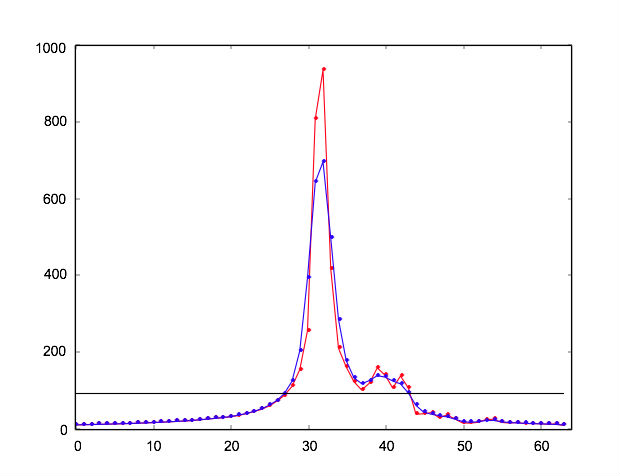
\includegraphics[height=60mm]{trees/gesture4-gauss1.jpg}
\end{center}

Für die effiziente und robuste Klassifizierung der Gesten bietet es sich weiterhin an, 
die Komplexität der generierten Eingabedaten zu reduzieren. Dazu wird in jedem Sample einer Geste 
auf der linken und rechten Seite des Referenztons die Anzahl der Amplituden des geglätteten Signals ermittelt, 
deren Wert größer als 10\% ist. Der daraus resultierende Graph zeigt dann für eine Geste die zeitliche 
Änderung der Amplitudenanteile um den Referenzton auf der linken und rechten Seite an. Dieser Graph ist in der folgenden 
Abbildung dargestellt, wobei die Anzahl der zum Referenzton gehörenden Amplituden aller Frequenzen unterhalb des
Referenztons in rot dargestellt sind, die Frequenzanteile oberhalb des Referenztons in blau:

\begin{center}
  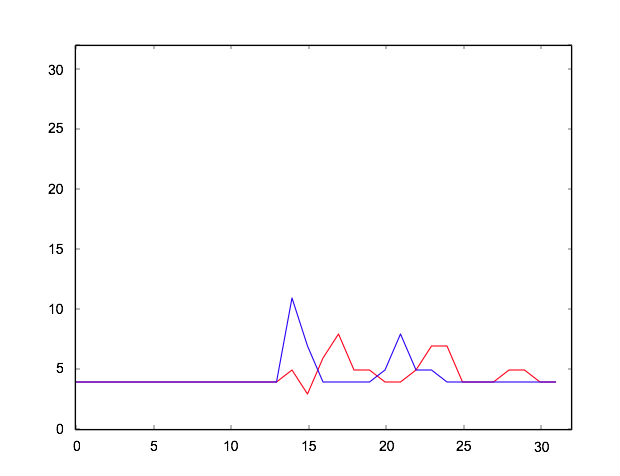
\includegraphics[height=60mm]{trees/gesture4-peaksize.jpg}
\end{center}

Bei der in der Grafik dargestellten Geste handelt es sich um einen \glqq Double-Tap\grqq\ , also eine Geste, bei der die Hand zwei mal 
hintereinander schnell auf den Monitor bzw. das Mikrofon zubewegt wird. Diese Geste äußert sich in jeweils zwei aufeinander folgenden 
Verschiebungen der Frequenzen nach rechts (auf den Monitor zu bewegen) und links (vom Monitor weg bewegen). 
Diese Charakteristik lässt sich in der Grafik erkennen, da die Anzahl der zum Referenzton gehörenden Frequenzanteile zunächst nach rechts (erster Peak blau) und dann nach links (zweiter Peak rot) ansteigt. Aufgrund des \glqq Double-Tap\grqq\  erfolgt diese 
Verschiebung zwei mal hintereinander, so dass insgesamt vier Ausschläge (zwei nach rechts und zwei nach links) zu erkennen sind. 
Somit kann in einem Schritt die Anzahl der Daten pro zu klassifizierender Geste von 32*64=2048 Amplitudenwerten 
auf 2*32=64 reduziert werden, wobei diese Werte keinen Rückschluss auf die genauen Frequenzanteile zulassen sondern 
ein Maß dafür sind, wie sich die Frequenzanteile ober- und unterhalb des Referenztons verändern.

Die daraus entstehenden Daten können in einem weiteren Schritt geglättet werden, da nur Amplitudenschwankungen ab einer gewissen 
Größe auf eine ausgeführte Bewegung schließen lassen. Dazu werden alle Schwankungen auf der rechten oder linken Seite entfernt, 
die unterhalb eines definierten Grenzwertes liegen. 
Die folgende Abbildung zeigt ein gefilterten Graph, in dem alle Ausschläge entfernt werden, die kleiner als 2 sind:

\begin{center}
  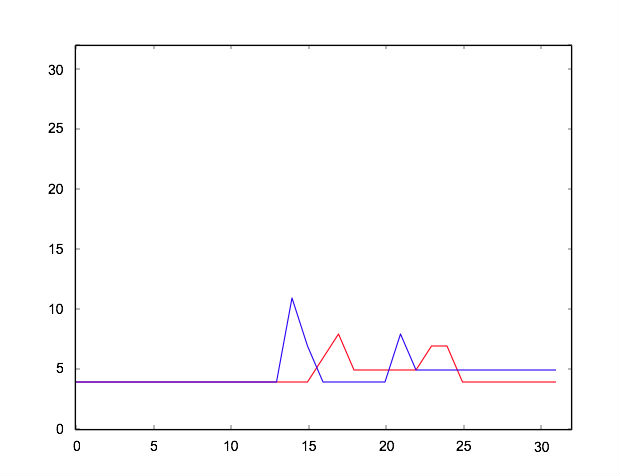
\includegraphics[height=60mm]{trees/gesture4-peaksize-smoothed.jpg}
\end{center}

In einen dritten Schritt werden die Amplitudenwechsel dahingehend weiter geglättet, indem zunächst die Anzahl der am häufigsten 
auftretenden Frequenzanteile auf der linken und rechten Seite vom Referenzton ermittelt werden. Anschließend werden alle Werte,
die in einem vorher definierten Bereich ober- oder unterhalb dieses Wertes liegen auf den am häufigsten vorkommenden Wert gesetzt.
Dieser Schritt ist in der folgenden Abbildung zu sehen, wobei alle Werte die +1 oder -1 um den häufigsten Wert verteilt sind 
auf den häufigsten Wert gesetzt wurden:

\begin{center}
  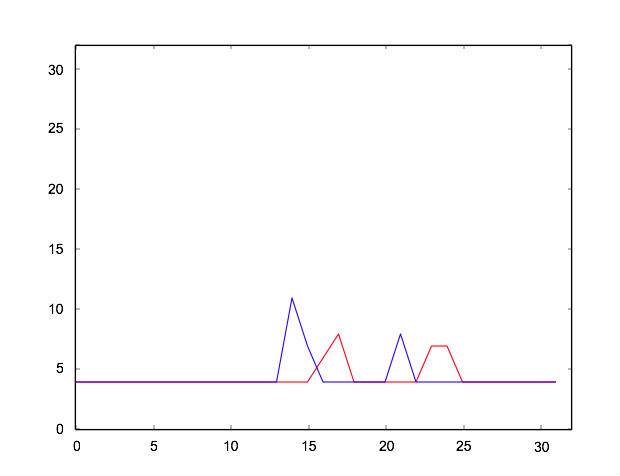
\includegraphics[height=60mm]{trees/gesture4-peaksize-smoothed2.jpg}
\end{center}


Stark vereinfacht unterscheiden sich die Gesten dahingehend, ob und auf welcher Seite 
eine Veränderung der Anzahl aller zum Referenzton gehörenden Frequenzanteile stattfindet. 
Weiterhin muss unterschieden werden, in welche Richtung sich diese Verschiebung ausbreitet. 
Sie kann beispielsweise von der rechten zur linken oder von der linken zur rechten Seite 
um den Referenzton wandern, sowie gleichzeitig auf beiden Seiten stattfinden. 
Ein Beispiel dafür zeigt die folgende Abbildung:

\begin{center} 
\label{fig:contrary}
  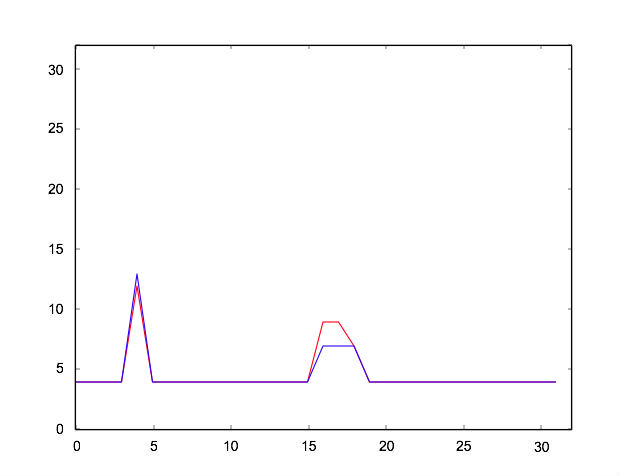
\includegraphics[height=60mm]{trees/gesture2-peaksize-smoothed2.jpg}
\end{center}

Bei der in der Grafik abgebildeten Geste handelt es sich um ein mit der rechten und linken Hand entgegengesetztes zu und 
wegbewegen von dem Monitor, so dass gleichzeitig auf der rechten und linken Seite eine Vergrößerung der 
zum Referenzton gehörenden Frequenzanteile entsteht, was sich auch in der Grafik ablesen lässt.
Diese Unterscheidungsmerkmale können sehr gut durch einen Entscheidungsbaum abgebildet werden. 
Dazu kann die Verschiebungsrichtung als Maß dienen, um die Eingabemenge zu unterteilen und 
somit eine Klassifizierung zu erreichen.

\subsubsection{Charakteristiken der Gesten} \label{charakteristiken}
Durch die Vorverarbeitung der Daten entstehen für die einzelnen Gesten Charakteristiken, anhand dessen sie unterschieden werden können. 

%\paragraph*{Right-to-left}

%\paragraph*{Top-to-bottom}

\paragraph*{Two-hands-contrary}
Die Geste \glqq Two-hands-contrary\grqq , dargestellt in Abbildung~\ref{fig:contrary}, zeigt üblicherweise je zwei gleichzeitige, also übereinanderliegende, Frequenzverschiebungen. Dies ist dadurch zu erklären, dass zur selben Zeit eine Bewegung auf das Aufnahmegerät zu und von diesem weg durchgeführt wird.

\begin{figure}[htbp] \centering
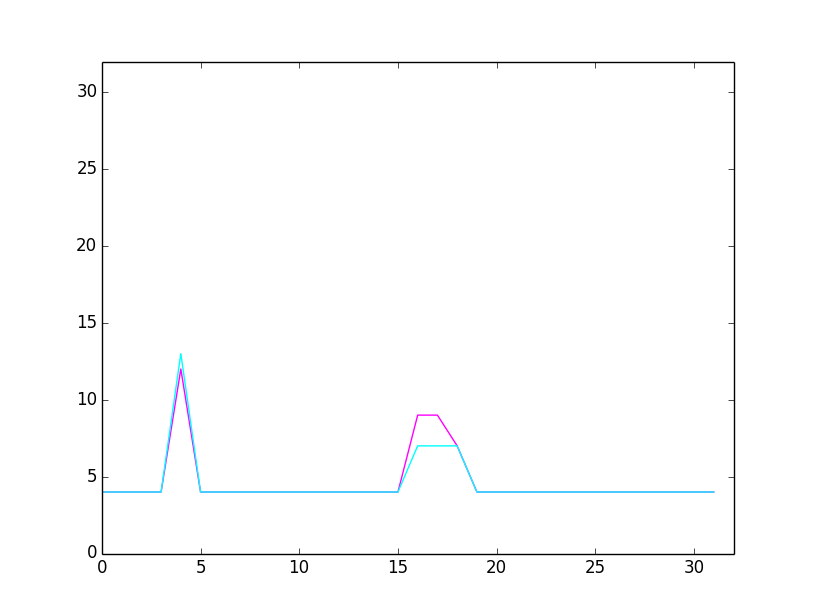
\includegraphics[height=60mm]{trees/contrary.png}
\caption{Two-hands-contrary}
\label{fig:contrary}
\end{figure}


\paragraph*{Single-Push}
Der \glqq Single-Push\grqq ist eine einfache Bewegung auf das Aufnahmegerät zu, sodass eine Frequenzverschiebung auf der rechten Seite des Frequenzspektrums festgestellt werden kann. Dies ist in Abbildung~\ref{fig:single_push} dargestellt.

\begin{figure}[htbp] \centering
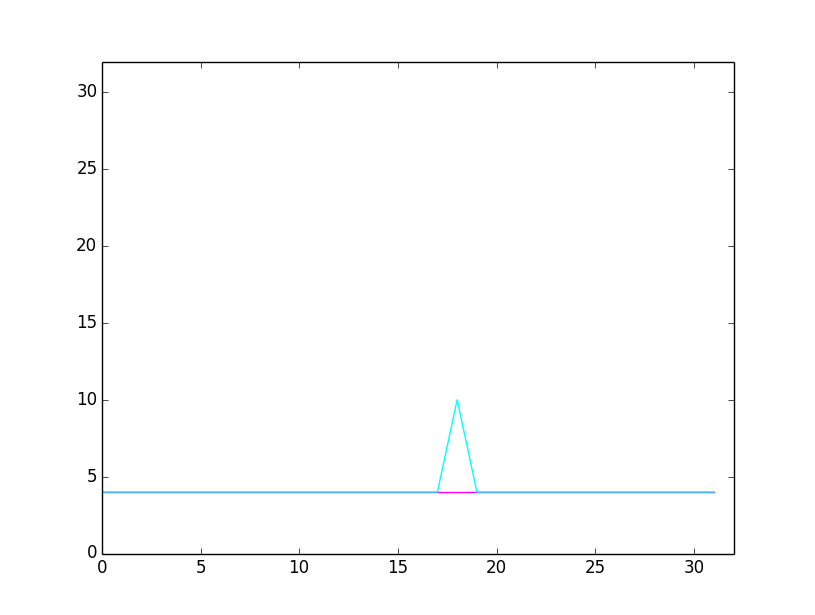
\includegraphics[height=60mm]{trees/single_push.png}
\caption{Single-Push}
\label{fig:single_push}
\end{figure}

\paragraph*{Double-Push}
Die Geste \glqq Double-Push\grqq ist in Abbildung~\ref{fig:double_push} abgebildet. Sie zeichnet sich aus durch in der Regel je zwei Verschiebungen auf der rechten und auf der linken Seite. Die Rechts-Links-Verschiebungen treten dabei kurz hintereinander auf und können sich auch teilweise überlappen. 

\begin{figure}[htbp] \centering
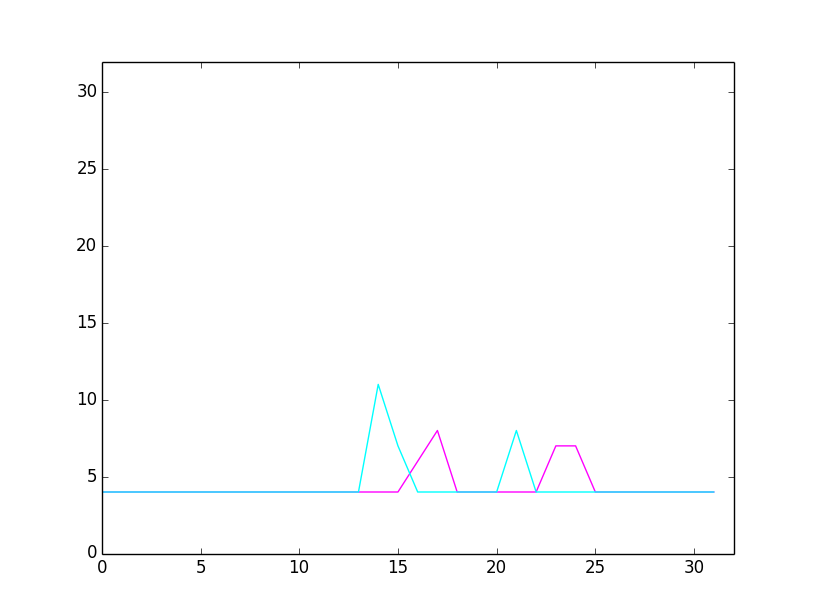
\includegraphics[height=60mm]{trees/double_push.png}
\caption{Double-Push}
\label{fig:double_push}
\end{figure}

\paragraph*{Nothing}
Um später Gesten live zu erkennen, muss auch definiert sein, wann keine Geste auftritt. In diesem Fall ist in Abbildung~\ref{fig:nothing} keine Frequenzverschiebung zu erkennen. Der Graph zeigt keinen Ausschlag.

\begin{figure}[htbp] \centering
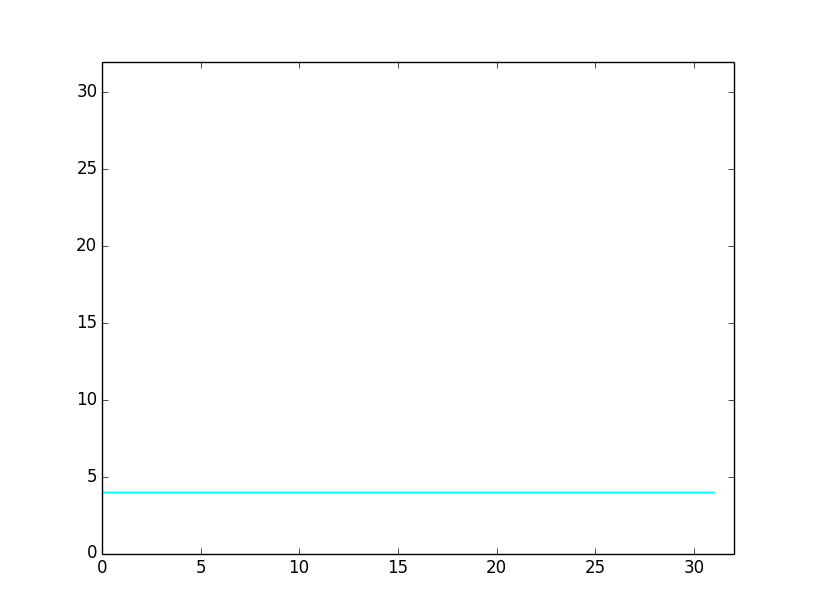
\includegraphics[height=60mm]{trees/nothing.png}
\caption{Keine Geste}
\label{fig:nothing}
\end{figure}

\subsection{Merkmalsextraktion}
Durch die Filterung und Glättung können nun die einzelnen Frequenzverschiebungen eindeutig identifiziert werden. Zudem ist in Abschnitt~\ref{charakteristiken} beschrieben, welche typische Gestalten der Graph für die verschiedenen Gesten annimmt. So lassen sich durch die Anordnung, Ausprägung und Aufkommen der Frequenzverschiebungen die unterschiedlichen Charakteristiken der einzelnen Gesten erkennen. Das Ziel der Merkmalsextraktion ist es, aus den 32 Datenpunkten weitere eindeutige Merkmale herauszuarbeiten um schließlich einen Merkmalsvektor mit überschaubarer Anzahl an Merkmalen zu generieren. Um dies zu realisieren, wurden folgende Eigenschaften der einzelnen Gesten untersucht:

\begin{itemize} 
\item Anzahl der Frequenzverschiebungen
\item Zeitliche Abfolge der Frequenzverschiebungen
\item Amplitudenunterschiede zwischen den Frequenzverschiebungen
\end{itemize}

\subsubsection*{Anzahl der Frequenzverschiebungen}
Die Anzahl der Frequenzverschiebung sagt bereits einiges über die Geste aus, wobei auch wichtig ist, ob die Frequenzverschiebungen im höheren oder niedrigeren Frequenzbereich liegen. Wie bereits in Abschnitt~\ref{} erwähnt, erzeugt eine Bewegung auf das Aufnahmegerät zu eine Frequenzverschiebung auf der rechten Seite, also eine Ausdehnung in Richtung der höheren Frequenzen. Durch das Bewegen vom Aufnahmegerät weg, erfolgt eine Frequenzverschiebung zur linken Seite, bzw. in Richtung der niedrigeren Frequenzen. 

Ein einfacher \glqq Single-Push\grqq\ erzeugt deshalb im optimalen Fall eine Frequenzverschiebung auf der rechten Seite des Peaks. Wird die Hand wieder zurückgezogen, tritt auch eine Frequenzverschiebung auf der linken Seite auf. Klar davon abgegrenzt werden kann beispielsweise die Geste \glqq Double-Push\grqq. Diese erzeugt mit dem Zurückziehen der Hand nach dem zweiten Push zwei Frequenzverschiebungen auf der linken und zwei auf der rechten Seite.

\subsubsection*{Zeitliche Abfolge der Frequenzverschiebungen}
Ein weiteres Merkmal einer Geste ist die zeitliche Abfolge der Frequenzverschiebungen. Ein \glqq Single-Push\grqq erzeugt zeitlich hintereinander erst eine Verschiebung rechts und dann eine Verschiebung links. Die Geste \glqq Two-hands-contrary\grqq , dargestellt in Abbildung~\ref{fig:contrary}, dagegen beschreibt die gleichzeitige gegensätzliche Bewegungen in Richtung des Aufnahmegeräts und von diesem weg. Somit tritt in diesem Fall gleichzeitig je eine Verschiebung nach rechts und links auf. 


\subsubsection*{Amplitudenunterschiede zwischen den Frequenzverschiebungen}
Die Gesten \glqq Single-Push\grqq und \glqq Right-to-Left-One-Hand\grqq unterscheiden sich in der zeitlichen Abfolge der Verschiebungen nicht. In beiden Fällen tritt erst eine Verschiebung rechts, dann links auf. Jedoch unterscheiden sich die Verschiebungen an sich. Bei \glqq Single-Push\grqq unterscheiden sich die beiden Verschiebungen im optimalen Fall nur dadurch, dass die eine Verschiebung links und die andere rechts vom Peak auftritt. Bei \glqq Right-to-Left-One-Hand\grqq dagegen ist die Amplitude der zweiten Verschiebung, links vom Peak, schwächer als die andere.

\subsection{Anpassung des Klassifikators}

\subsection{Implementierung}

Die Bibliothek \textit{sklearn}~\cite{sklearn} stellt mit dem Modul \textit{sklearn.ensemble}~\cite{sklearn.ensemble} einige hilfreiche Klassen und Methoden zur Klassifikation bereit.

\subsection{Training}

\subsection{Evaluation}

\subsection{Fazit}


